\section{PCB Specifications}

\begin{table}[h!]
\centering
\begin{tabular}{l|l}
\toprule
\textbf{Parameter} & \textbf{Specification} \\ \bottomrule
Substrate Material & \textcolor{orange}{\hyperref[subsec:selectedPCBsubstrate]{Rogers TMM10i}} \\
Conductive Layer & \textcolor{orange}{Copper + Gold Plating (Non-Magnetic)}\footnotemark \\
Target Impedance & 50 $\Omega$ \\
Frequency Range & 9 kHz -- 18 GHz\ \footnotemark\\
% PCB design Tool & Altume \\
connector type & SMP (Amphenol RF 925-NM196J-51P non-magnetic) \\
connector count & one version with 2 ports and one with 6 ports \\ 
Transmission Line & Coplanar Waveguide (CPW) \\
\quad Substrate Height ($h$) & \textcolor{orange}{0.030” (0.762mm) \hyperref[fig:RogersTTMstandardThicknesses]{[Rogers TTM standard]}} \\
\quad Trace Width ($w$) & \textcolor{red}{Calculate via CPW model} \\
\quad Gap Width ($s$) & \textcolor{red}{Calculate via CPW model} \\
Chip Mounting Cavity &\textcolor{orange}{$6.3\times6.3\times0.38\  mm^3$\ \footnotemark}\\
Manufacturer & \textcolor{red}{\textbf{??}} \\
\bottomrule
\end{tabular}
\end{table}
\footnotetext[\numexpr\value{footnote}-2]{make sure that the adhesion layer is not magnetic -- check EPIG (Electroless Palladium Immersion Gold)}
\footnotetext[\numexpr\value{footnote}-1]{18GHz is the limit of the SMP connectors we have. option to buy \href{https://www.svmicrowave.com/smpm-male-non-magnetic-pcb-surface-mount-connector-fd}{up-to 20GHz connector}.}
\footnotetext[\numexpr\value{footnote}]{or drill through}

\begin{figure}[h]
    \centering
    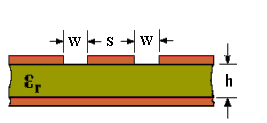
\includegraphics[width=0.5\linewidth]{tex/CPW.png}
\end{figure}
